\documentclass[a4paper,twoside]{article}
\usepackage{blindtext}  
\usepackage{geometry}

% Chinese support
\usepackage[UTF8, scheme = plain]{ctex}

% Page margin layout
\geometry{left=2.3cm,right=2cm,top=2.5cm,bottom=2.0cm}


\usepackage{listings}
\usepackage{xcolor}
\usepackage{geometry}
\usepackage{amsmath}
\usepackage{float}
\usepackage{hyperref}

\usepackage{graphics}
\usepackage{graphicx}
\usepackage{epsfig}
\usepackage{float}
\usepackage{wrapfig}

\usepackage{algorithm}
\usepackage[noend]{algpseudocode}

\usepackage{booktabs}
\usepackage{threeparttable}
\usepackage{longtable}
\usepackage{listings}
\usepackage{tikz}
\usepackage{multicol}

\usepackage{caption}
\usepackage{subcaption}

% cite package, to clean up citations in the main text. Do not remove.
\usepackage{cite}

\usepackage{color,xcolor}

%% The amssymb package provides various useful mathematical symbols
\usepackage{amssymb}
%% The amsthm package provides extended theorem environments
\usepackage{amsthm}
\usepackage{amsfonts}
\usepackage{enumerate}
\usepackage{enumitem}
\usepackage{listings}

\usepackage{textcomp}

\usepackage{indentfirst}
\setlength{\parindent}{2em} % Make two letter space in the first paragraph
\usepackage{setspace}
\linespread{1.5} % Line spacing setting
\usepackage{siunitx}
\setlength{\parskip}{0.5em} % Paragraph spacing setting

% \usepackage[contents =22920202204622, scale = 10, color = black, angle = 50, opacity = .10]{background}

\renewcommand{\figurename}{图}
\renewcommand{\lstlistingname}{代码} 
\renewcommand{\tablename}{表格}
\renewcommand{\contentsname}{目录}
\floatname{algorithm}{算法}

\graphicspath{ {images/} }

%%%%%%%%%%%%%
\newcommand{\StudentNumber}{22920202204622}  % Fill your student number here
\newcommand{\StudentName}{熊恪峥}  % Replace your name here
\newcommand{\PaperTitle}{实验(三)}  % Change your paper title here
\newcommand{\PaperType}{计算机网络} % Replace the type of your report here
\newcommand{\Date}{2022年11月3日}
\newcommand{\College}{信息学院}
\newcommand{\CourseName}{计算机网络}
%%%%%%%%%%%%%

%% Page header and footer setting
\usepackage{fancyhdr}
\usepackage{lastpage}
\pagestyle{fancy}
\fancyhf{}
% This requires the document to be twoside
\fancyhead[LO]{\texttt{\StudentName }}
\fancyhead[LE]{\texttt{\StudentNumber}}
\fancyhead[C]{\texttt{\PaperTitle }}
\fancyhead[R]{\texttt{第{\thepage}页,共\pageref*{LastPage}页}}


\title{\PaperTitle}
\author{\StudentName}
\date{\Date}

\lstset{
	basicstyle          =   \sffamily,          % 基本代码风格
	keywordstyle        =   \bfseries,          % 关键字风格
	commentstyle        =   \rmfamily\itshape,  % 注释的风格,斜体
	stringstyle         =   \ttfamily,  % 字符串风格
	flexiblecolumns,                % 别问为什么,加上这个
	numbers             =   left,   % 行号的位置在左边
	showspaces          =   false,  % 是否显示空格,显示了有点乱,所以不现实了
	numberstyle         =   \zihao{-5}\ttfamily,    % 行号的样式,小五号,tt等宽字体
	showstringspaces    =   false,
	captionpos          =   t,      % 这段代码的名字所呈现的位置,t指的是top上面
	frame               =   lrtb,   % 显示边框
}

\lstdefinestyle{PythonStyle}{
	language        =   Python, % 语言选Python
	basicstyle      =   \zihao{-5}\ttfamily,
	numberstyle     =   \zihao{-5}\ttfamily,
	keywordstyle    =   \color{blue},
	keywordstyle    =   [2] \color{teal},
	stringstyle     =   \color{magenta},
	commentstyle    =   \color{red}\ttfamily,
	breaklines      =   true,   % 自动换行,建议不要写太长的行
	columns         =   fixed,  % 如果不加这一句,字间距就不固定,很丑,必须加
	basewidth       =   0.5em,
}

\definecolor{keycolor}{RGB}{172, 42, 42}
\definecolor{mbleu}{RGB}{64,96,127}
\definecolor{vimvert}{RGB}{46, 139, 87}

\lstdefinestyle{MakefileBaseStyle}{
basicstyle=\ttfamily\scriptsize\color{black!90},%
stringstyle=\itshape\color{magenta},%
showstringspaces=false,%
keywordstyle=\bfseries\color{keycolor},%
commentstyle=\color{blue}\slshape,%
framexleftmargin=1mm,%
backgroundcolor=\color{black!2},%
}

\lstdefinestyle{MakefileStyle}{
	otherkeywords={.SUFFIXES},
	morekeywords={SUFFIX, CPP_,},
	moredelim=[is][\color{mbleu}]{/*}{*/},
	style=MakefileBaseStyle,%
	morecomment=[l][commentstyle]{\#},%
	emphstyle={\color{vimvert}},%
	moredelim=[s][\color{vimvert}]{\$(}{)}%
}

\lstdefinestyle{CppStyle}{
	language        =   c++,
	basicstyle      =   \zihao{-5}\ttfamily,
	numberstyle     =   \zihao{-5}\ttfamily,
	keywordstyle    =   \color{blue},
	keywordstyle    =   [2] \color{teal},
	stringstyle     =   \color{magenta},
	commentstyle    =   \color{red}\ttfamily,
	breaklines      =   true,   % 自动换行,建议不要写太长的行
	columns         =   fixed,  % 如果不加这一句,字间距就不固定,很丑,必须加
	basewidth       =   0.5em,
}

\algnewcommand\algorithmicinput{\textbf{Input:}}
\algnewcommand\algorithmicoutput{\textbf{Output:}}
\algnewcommand\Input{\item[\algorithmicinput]}%
\algnewcommand\Output{\item[\algorithmicoutput]}%

\usetikzlibrary{positioning, shapes.geometric}

% 流程图定义基本形状
\tikzstyle{startstop} = [rectangle, rounded corners, minimum width = 2cm, minimum height=1cm,text centered, draw = black]
\tikzstyle{io} = [trapezium, trapezium left angle=70, trapezium right angle=110, minimum width=2cm, minimum height=1cm, text centered, draw=black]
\tikzstyle{process} = [rectangle, minimum width=3cm, minimum height=1cm, text centered, draw=black]
\tikzstyle{decision} = [diamond, aspect = 3, text centered, draw=black]
% 箭头形式
\tikzstyle{arrow} = [->,>=stealth]

\newtheorem{assumption}{Assumption}[section]

\begin{document}
	
%%%%%%%%%%%%%%%%%%%%%%%%%%%%%%%%%%%%%%%%%%%%
\makeatletter % change default title style
\renewcommand*\maketitle{%
	\begin{center} 
		\bfseries  % title 
		{\LARGE \@title \par}  % LARGE typesetting
		\vskip 1em  %  margin 1em
		{\global\let\author\@empty}  % no author information
		{\global\let\date\@empty}  % no date
		\thispagestyle{empty}   %  empty page style
	\end{center}%
	\setcounter{footnote}{0}%
}
\makeatother
%%%%%%%%%%%%%%%%%%%%%%%%%%%%%%%%%%%%%%%%%%%%
	
	
\thispagestyle{empty}

\vspace*{1cm}

\begin{figure}[h]
	\centering
	
\includegraphics[width=4.0cm]{logo.png}
\end{figure}

\vspace*{1cm}

\begin{center}
	\Huge{\textbf{\PaperType}}
	
	\Large{\PaperTitle}
\end{center}

\vspace*{1cm}

\begin{table}[h]
	\centering	
	\begin{Large}
		\renewcommand{\arraystretch}{1.5}
		\begin{tabular}{p{3cm} p{5cm}<{\centering}}
			姓\qquad 名 & \StudentName  \\
			\hline
			学\qquad号 & \StudentNumber \\
			\hline
			日\qquad期 & \Date  \\
			\hline
			学\qquad院 & \College  \\
			\hline
			课程名称 & \CourseName  \\
			\hline
		\end{tabular}
	\end{Large}
\end{table}

\newpage

\title{
	\Large{\textcolor{black}{\PaperTitle}}
}
	
	
\maketitle
	
\tableofcontents
 
\newpage
\setcounter{page}{1}

\begin{spacing}{1.2}

\section{编译和运行代码}

实验代码在以下环境中进行了编译和运行:

\begin{itemize}
	\item 操作系统:\texttt{Ubuntu 22.04 (on Windows Subsystem for Linux)}
	\item 编译器:\texttt{GCC 11.3.0}
	\item CMake:\texttt{3.22.1}
\end{itemize}

为了编译代码,需要使用CMake,在项目目录下建立目录build,然后依次运行:

\begin{enumerate}
	\item cd build 
	\item cmake .. 
	\item make 
\end{enumerate}

就可以得到server和client两个可执行文件。运行方式都是\textbf{"可执行文件名 \ IP \ PORT"}。分别
为程序指定IP和端口。

\section{完善Socket客户机和服务器}

\subsection{程序实现}

\subsubsection{通过命令行参数指定IP和端口}

首先,为了实现通过参数指定服务器IP和端口,需要处理命令行参数。
先检查主函数的$argc$,如果不是3,说明参数不对,打印提示信息并退出。如代码~\ref{code:argc}。

\begin{lstlisting}[numbers=left,style=CppStyle,caption=检查$argc$,label={code:argc}]
if (argc != 3)
{
	printf("Usage: %s <IP> <PORT>", argv[0]);
	return -1;
}
\end{lstlisting}

然后在构造$sever_addr$结构体的时候根据输入的IP和端口号进行赋值。用户输入的端口号是一个数字字符串,首先使用
$atoi$转换成整数,然后通过$htons$转换成网络字节序。而用户输入的IP地址是一个点分十进制字符串,需要使用$inet\_aton$转换成
一个整形。如代码~\ref{code:addr}。

\begin{lstlisting}[numbers=left,style=CppStyle,caption=构造$sever_addr$结构体,label={code:addr}]
server_addr.sin_port = htons(atoi(argv[2]));
inet_aton(argv[1], &server_addr.sin_addr);
\end{lstlisting}

这样,就可以通过命令行参数指定服务器IP和端口了。

\subsubsection{服务器端处理SIGINT信号}

由于服务器端使用$bind$绑定了端口,如果退出时没有正确释放资源,端口就会被占用。之后的运行就需要指定其他端口,造成了资源的浪费。
使用Ctrl+C退出时,服务器端会收到SIGINT信号,可以在主函数中捕获这个信号,然后在信号处理函数中调用$close$释放资源。
否的程序会直接退出,因而无法释放资源,造成问题。如代码~\ref{code:sigint}。

\begin{lstlisting}[numbers=left,style=CppStyle,caption=捕获SIGINT信号,label={code:sigint}]
void release_socket(int signo)
{
	close(server_sock_listen);
	exit(-1);
}

// in int main()
signal(SIGINT, release_socket);
\end{lstlisting}

\subsubsection{为Socket添加错误处理}

为了给Socket添加错误处理,需要在每次调用Socket函数的时候检查返回值,
Socket如果返回-1,说明调用失败,那么就打印错误信息并退出。在退出时需要注意释放已经获取的资源。
为了更好地解决资源释放的问题,可以采用Linux内核中“向下goto”的方式跳转到相应的异常处理部分。
这种方式是对goto的一种合理使用。

正如Linux Device Drivers Book中\cite{corbet2005linux}所说的:

\textit{
	The goto is \emph{useful} in a routine that allocates resources, performs operations on those resources, 
	and then deallocates the resources. With a goto, you can clean up in one section of the code. 
	The goto \emph{reduces the likelihood of your forgetting to deallocate the resources in each place you detect an error.}
}

虽然goto语句在C语言中被认为是不好的编程风格\cite{dijkstra1968letters},
但是在错误处理这种特殊场景中是一种正确的使用。这种风格的例子如代码~\ref{code:goto}。

\begin{lstlisting}[numbers=left,style=CppStyle,caption=向下goto,label={code:goto}]
int foo(int bar)
{
    int return_value = 0;
    if (!do_something( bar )) {
        goto error_1;
    }
    if (!init_stuff( bar )) {
        goto error_2;
    }
    if (!prepare_stuff( bar )) {
        goto error_3;
    }
    return_value = do_the_thing( bar );
error_3:
    cleanup_3();
error_2:
    cleanup_2();
error_1:
    cleanup_1();
    return return_value;
}
\end{lstlisting}

在\nameref{sec:code}中,代码~\ref{code:client}、代码~\ref{code:server_iter}、代码~\ref{code:server_parl}
都用了这种方式来处理多个fd的释放。

\subsubsection{允许用户输入字符串}

为了允许用户输入字符串,可以开辟一定的缓冲区,然后使用$fgets$输入任意字符。使用$fgets$的好处是它可以指定缓冲区长度,可以防止
缓冲区溢出,更为安全。另外,使用$fgets$输入的字符串末尾会有一个$'\backslash 0'$,所以不需要再手动添加$'\backslash 0'$。也不会因为忘记添加
该符号而造成问题。

\subsubsection{使用bye退出}

服务器端需要把处理和返回消息的部分加入一个循环中,直到收到bye消息才退出。
客户端在服务器返回bye消息后再释放资源退出。

\subsubsection{将服务器端改为迭代服务器}

迭代服务器可以依次对所有的客户机进行服务。在服务器端,需要使用一个循环来接收客户机的连接请求。
所有的请求都在服务器的单个进程中依次处理。为此,可以把服务器端的代码改为如代码~\ref{code:server_iter}所示。
将$accept$调用以及对消息的处理放进一个循环中,这样就可以依次接收多个客户机的连接请求了。
当客户机输入bye的时候进入下一次循环,服务器端就会关闭当前的连接,然后$accept$等待下一个客户机的连接请求。

\subsection{客户机和服务器的运行情况}

如图~\ref{fig:iter},运行迭代版的服务器,用4个客户端进行连接。可以看到,服务器端只能依次处理4个客户端的请求。
每次只有一个服务端能得到处理。当该客户端输入bye结束后,下一个客户端才能得到处理。

\begin{figure}[htb]
	\centering
	\caption{迭代版的服务器}
	\label{fig:iter}
	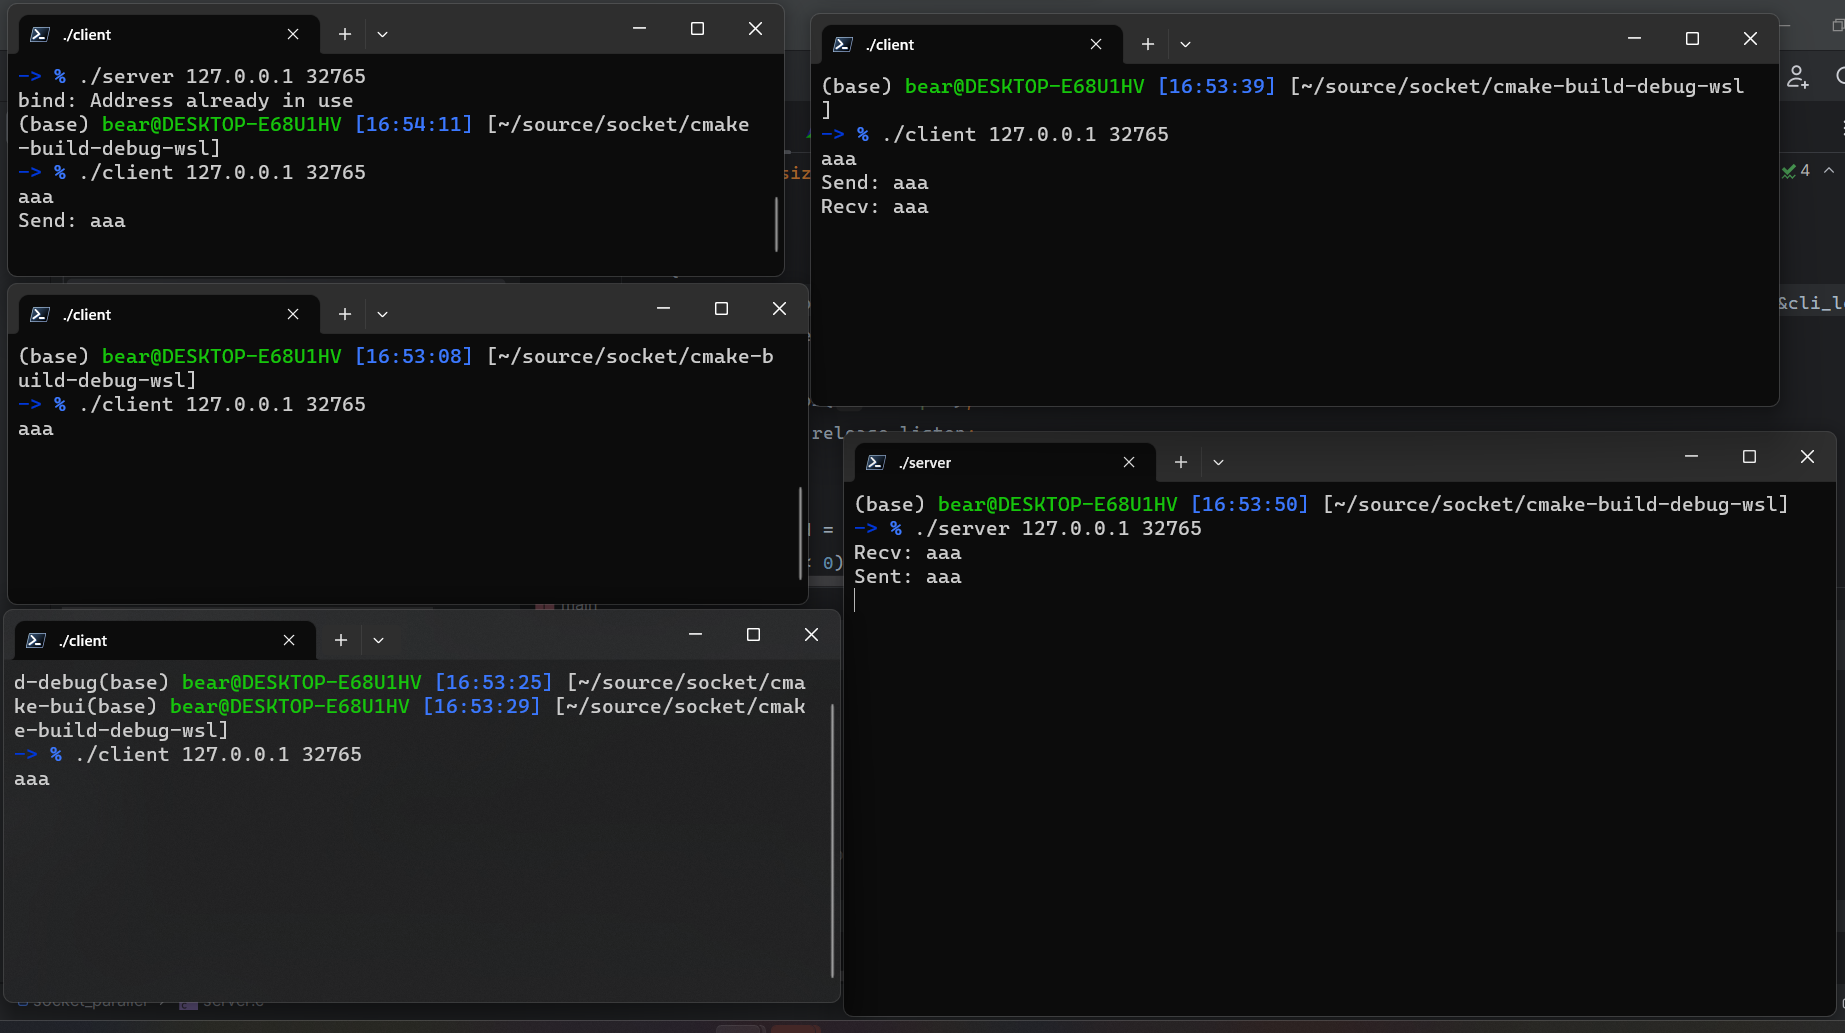
\includegraphics[width=0.6\textwidth]{server_iter.png}
\end{figure}

\subsection{Server端的Backlog}

在服务器端,Socket建立连接主要分为以下几步:

\begin{enumerate}
	\item 将TCP状态设置为LISTEN状态,开启监听客户端的连接请求
	\item 收到客户端发送的SYN报文后,TCP状态切换为SYN RECEIVED,并发送SYN ACK报文
	\item 收到客户端发送的ACK报文后,TCP三次握手完成,状态切换为ESTABLISHED
\end{enumerate}

其中,第一步通过调用$listen$完成。其中$backlog$是已完成的连接队列(ESTABLISHED)与未完成连接队列(SYN\_RCVD)之和的上限。
将参数设置为0和1的运行结果使用netstat进行统计,如图~\ref{fig:backlog}所示。


\begin{figure}[htbp]
	\centering
	\caption{不同的$backlog$}
	\label{fig:acc}
	\begin{subfigure}{0.4\textwidth}
		\centering
		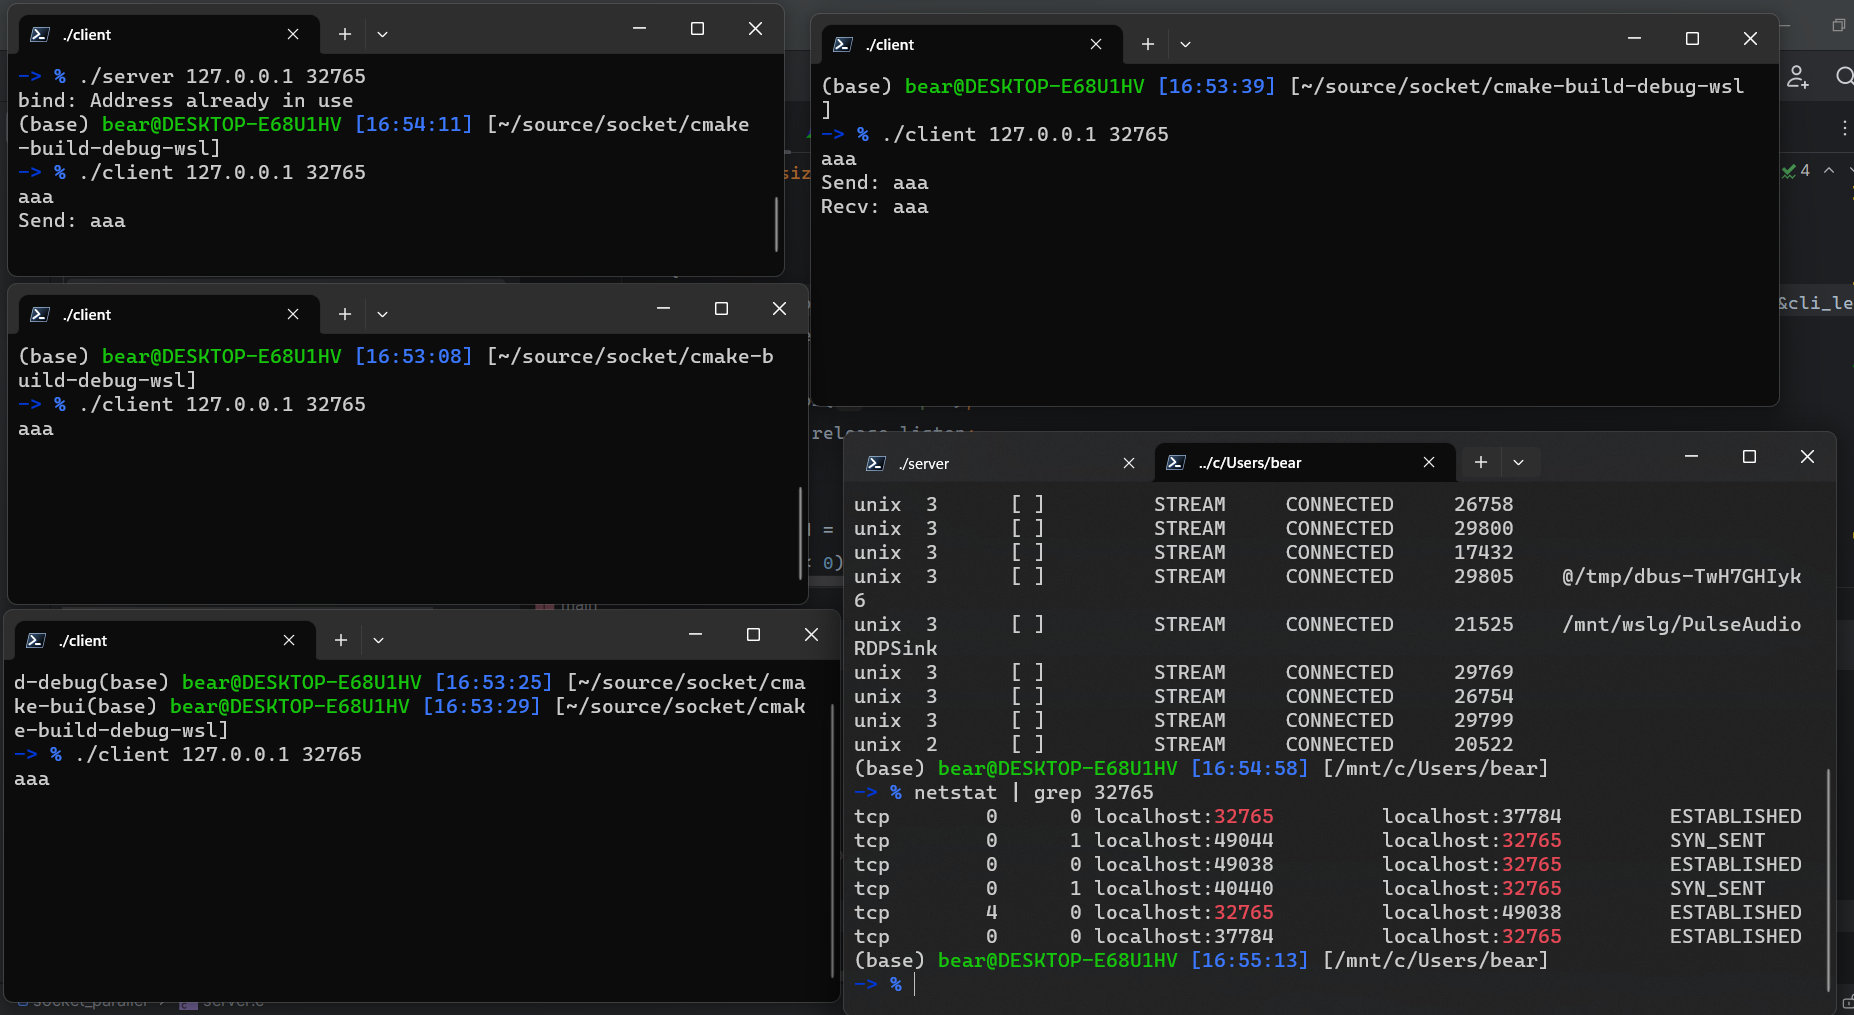
\includegraphics[width=\textwidth]{iter_bl0.png}
		\caption{$backlog=0$}
		\label{fig:bl0}
	\end{subfigure}
	\begin{subfigure}{0.4\textwidth}
		\centering
		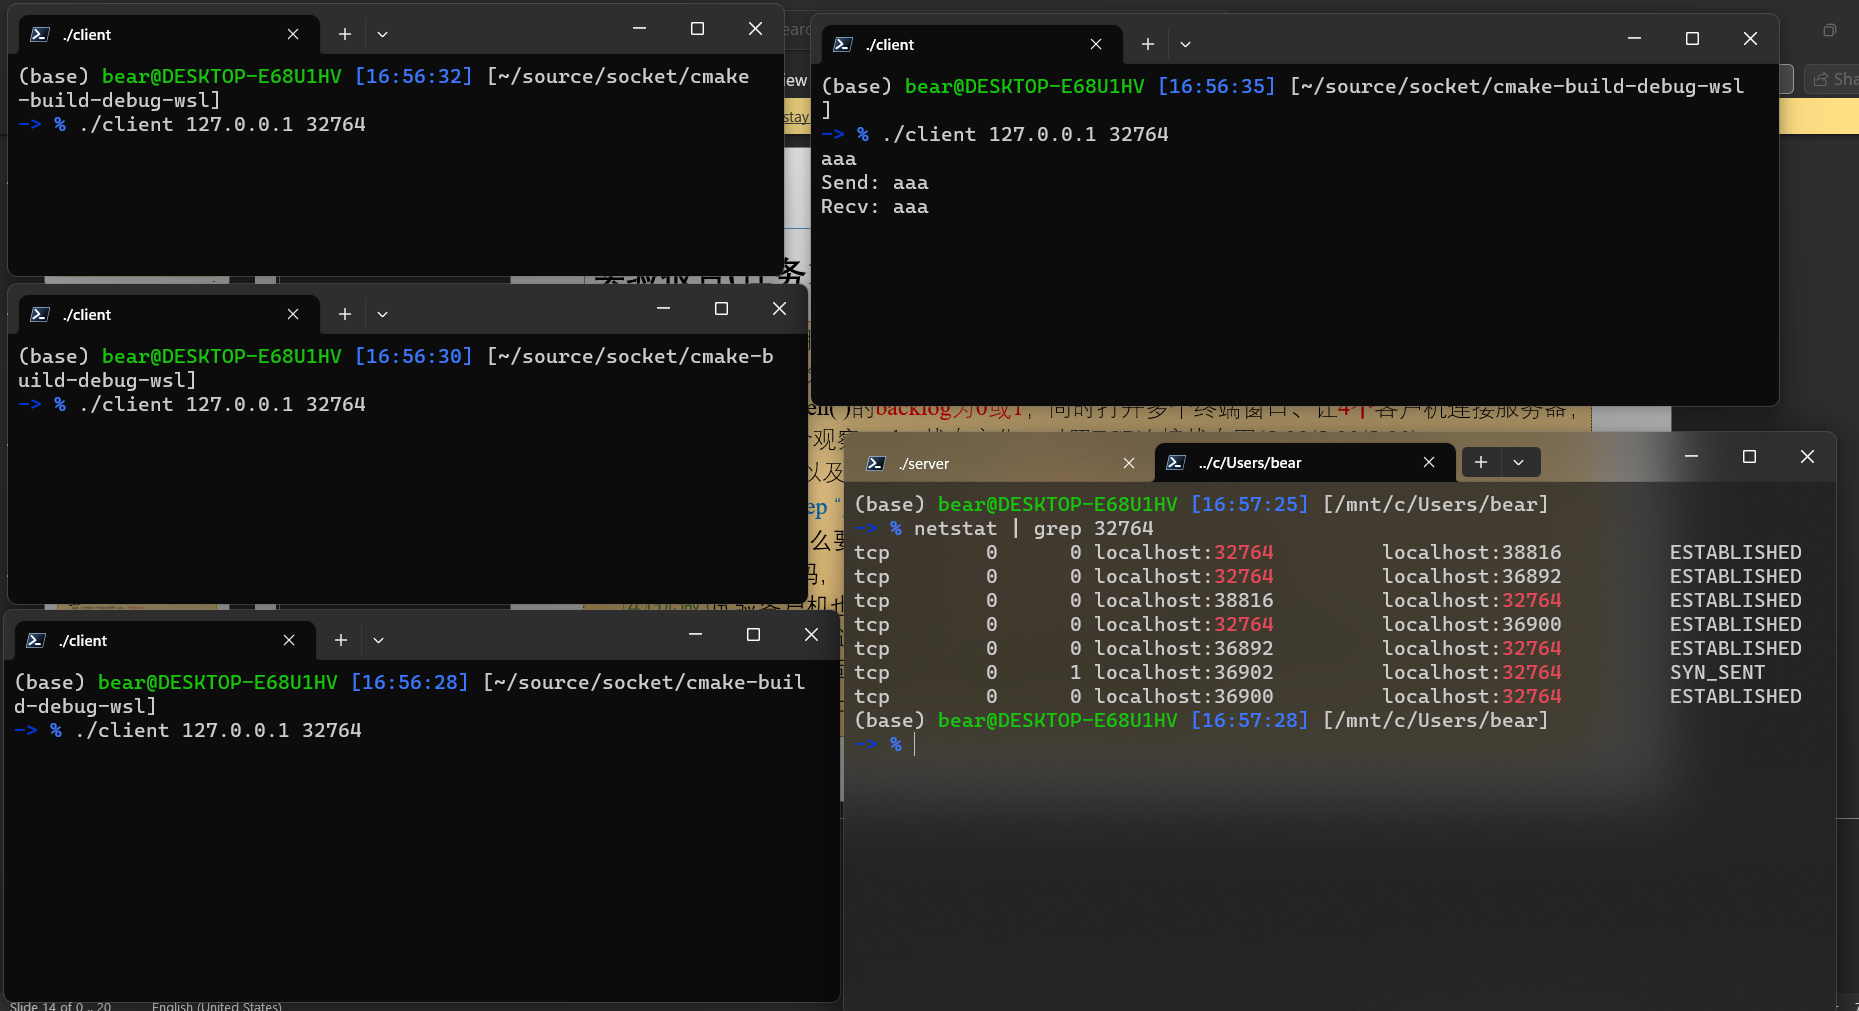
\includegraphics[width=\textwidth]{iter_bl1.png}
		\caption{$backlog=1$}
		\label{fig:bl1}
	\end{subfigure}
\end{figure}

可以发现,对于4个尝试建立连接的客户端,当$backlog=0$时,使用netstat可以发现有
2对连接处于ESTABLISHED状态,当$backlog=1$时,使用netstat则有3对。可见,
$backlog$确实限制了服务器端的连接数。

\section{TCP并发服务器}


\subsection{程序实现}

为了实现多进程,需要使用$fork$系统调用。首先,为了方便建立多个连接,需要将$listen$的
参数$n$设置成较大的数,例如5。然后循环进行$accept$调用,接收客户机的连接请求。

一旦接受了客户机的连接请求,就需要创建一个子进程来处理客户机的请求。在父进程中,需要关闭服务器端的套接字,
在子进程中,执行正常的TCP Echo Server的执行流程。当收到Bye结束时,子进程需要关闭套接字,释放资源,然后退出。

判断父进程和子进程通过$fork$的返回值来判断。如果$fork$返回值为0,说明是子进程,如果返回值大于0,说明是父进程。
代码见\nameref{sec:code}中的代码~\ref{code:server_parl}。

\subsection{并发服务器的运行情况}

运行并发服务器,结果如图~\ref{fig:parl}所示。四个客户端都能分别发送消息,服务器端也能正常接收。

\begin{figure}[htb]
	\centering
	\caption{并发的服务器}
	\label{fig:parl}
	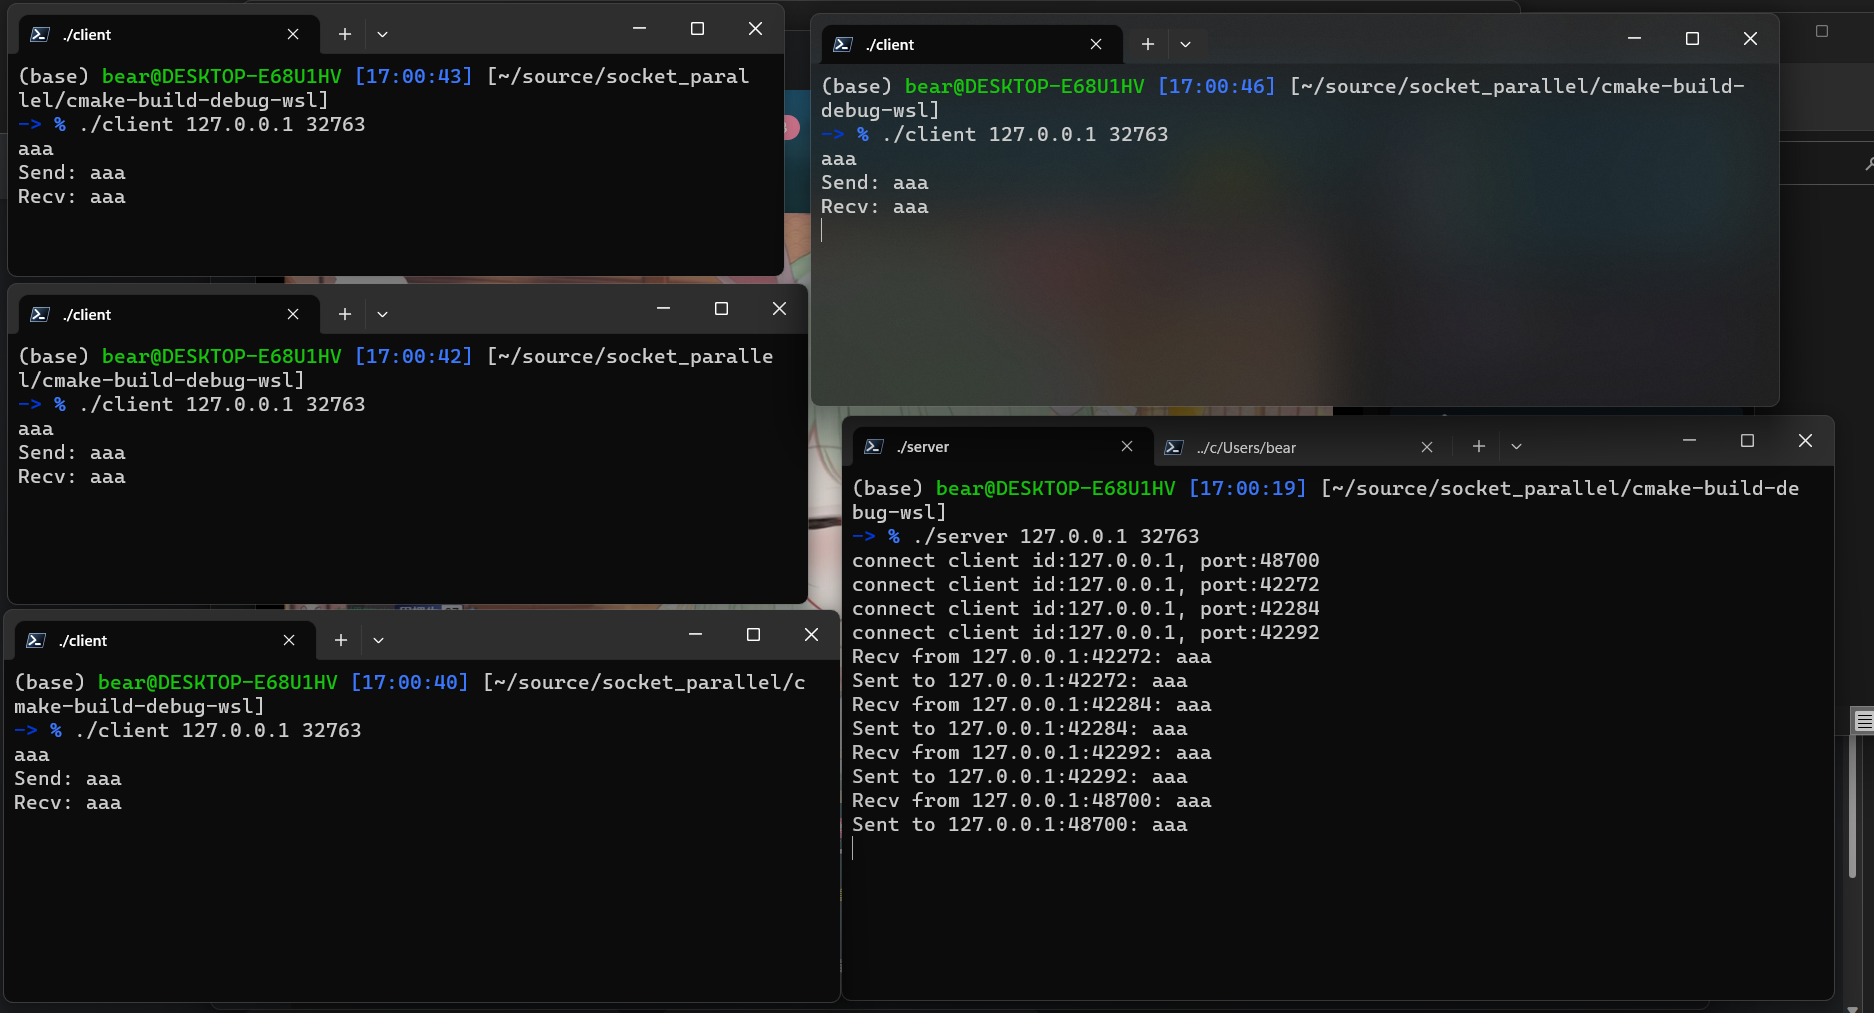
\includegraphics[width=0.6\textwidth]{para.png}
\end{figure}

\subsection{父进程分支中是否需要关闭Socket}

从结论上来说,\emph{父进程分支中必须关闭Socket},否则会造成系统资源的浪费。

\subsubsection{理论分析}

为了分析这个问题,首先要理解$fork$的功能。$fork$的作用是创建一个新的进程,新的进程是原进程的一个副本。
这个系统调用是所有类Unix系统进程模型的中心。因此我们可以通过分析一个相对简单的Unix操作系统XV6的$fork$系统调用实现
来分析这个问题。

XV6的$fork$系统调用实现如代码~\ref{code:fork}所示。在$fork$系统调用中,首先调用了$allocproc$函数来分配一个进程结构体。
然后对这个进程结构体进行初始化,包括设置进程的状态,设置进程的父进程,设置进程的内存空间等。此时,父进程的整个内存内容都通过
$copyuvm$进行了复制,然后所有父进程打开的文件都通过$filedup$进行了复制。最后,子进程$trapframe$的$eax$设置成了1,
这样在子进程中$fork$的返回值就会成为0。

\begin{lstlisting}[numbers=left,style=CppStyle,caption={XV6的$fork$系统调用实现},label={code:fork}]

int
fork(void)
{
  int i, pid;
  struct proc *np;

  // Allocate process.
  if((np = allocproc()) == 0)
    return -1;

  // Copy process state from p.
  if((np->pgdir = copyuvm(proc->pgdir, proc->sz)) == 0){
    kfree(np->kstack);
    np->kstack = 0;
    np->state = UNUSED;
    return -1;
  }
  np->sz = proc->sz;
  np->parent = proc;
  *np->tf = *proc->tf;
  np->mode = proc->mode;
  np->parentfds = proc->parentfds;

  // Clear %eax so that fork returns 0 in the child.
  np->tf->eax = 0;

  for(i = 0; i < NOFILE; i++)
    if(proc->ofile[i])
      np->ofile[i] = filedup(proc->ofile[i]);
  np->cwd = idup(proc->cwd);
  np->thr = proc->thr;

  pid = np->pid;
  np->state = RUNNABLE;
  safestrcpy(np->name, proc->name, sizeof(proc->name));
  return pid;
}
\end{lstlisting}

由于Socket API的设计遵从UNIX“一切皆文件”的设计理念,因此Socket调用也是基于文件系统的,打开一个Socket就会创建
一个文件描述符。因此,为了确认是否需要在父进程中关闭相应的Socket,需要进一步探究$fork$系统调用中的$filedup$函数的实现。

$filedup$函数的实现如代码~\ref{code:filedup}所示。可见,复制文件描述符的时候,只是将文件描述符的引用计数加1,而不是
真正意义上的复制。

\begin{lstlisting}[numbers=left,style=CppStyle,caption={$filedup$函数的实现},label={code:filedup}]
struct file *
filedup(struct file *f)
{
	acquire(&ftable.lock);
	if (f->ref < 1)
	{
		panic("filedup");
	}
	f->ref++;
	release(&ftable.lock);
	return f;
}
\end{lstlisting}

而当关闭文件的时候,系统会检查文件的引用计数,如果引用计数为0,才会真正释放文件,否则不进行任何操作。
如代码~\ref{code:fileclose}所示。

\begin{lstlisting}[numbers=left,style=CppStyle,caption={$fileclose$函数的实现},label={code:fileclose}]
void
fileclose(struct file *f)
{
	... 
	if (--f->ref > 0)
	{
		release(&ftable.lock);
		return;
	}
	...
}
\end{lstlisting}

这样一来,如果父进程中的Socket没有被关闭,那么子进程中对Socket关闭时,内核首先对相应文件管理
结构的引用计数-1,然后发现引用计数不为0,因此不会真正释放文件。这样一来,子进程中的Socket就会一直保持打开状态,
没有被关闭。因此,父进程中如果不关闭该Socket,就会对系统资源产生浪费,因为这个Socket将永远不会
得到关闭。

由于类UNIX操作系统的$fork$都有相同的功能,所以这一分析可以很好地推广到常见的Linux内核中。当$fork$发生时,
相应的描述符会发生逻辑上的复制,所以如果父进程不关闭相应的Socket,就会造成资源的浪费。

\subsubsection{实验验证}

使用netstat工具来对是否关闭Socket的服务器进行信息的获取,如图~\ref{fig:closeornot}。

\begin{figure}[htbp]
	\centering
	\caption{是否关闭}
	\label{fig:acc}
	\begin{subfigure}{0.4\textwidth}
		\centering
		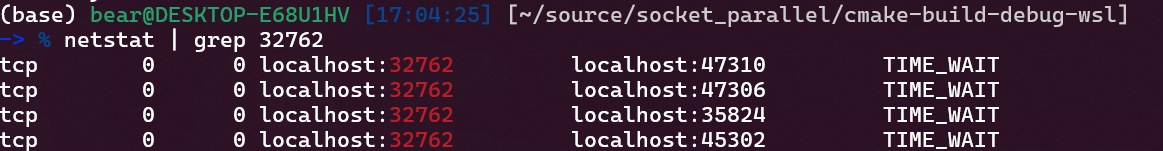
\includegraphics[width=\textwidth]{close.png}
		\caption{关闭}
		\label{fig:close}
	\end{subfigure}
	\begin{subfigure}{0.4\textwidth}
		\centering
		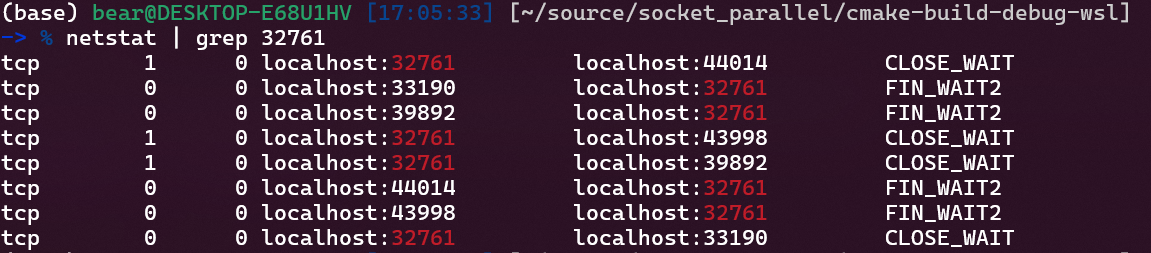
\includegraphics[width=\textwidth]{noclose.png}
		\caption{不关闭}
		\label{fig:noclose}
	\end{subfigure}
\end{figure}

可以发现如果不关闭,那么在进程结束之后也会残留CLOSE\_WAIT状态的连接。这大大浪费了系统资源。
因此,需要在父进程中关闭相应的Socket。

\section{实验总结}

通过这次实验,我学习了如何调用Socket API通过TCP连接收发网络数据。并实现了迭代版和并发版的不同服务器端。
在实验过程中,我学习了如何使用netstat
工具获得所需要的信息。同时,通过理论分析和实验验证,我学到了在$fork$之后,必须关闭父进程中的Socket这一
原则。这一原则对于防止网络程序对系统资源的浪费有很大的帮助。

\appendix
\clearpage
\section*{参考文献}
\addcontentsline{toc}{part}{参考文献}

\bibliographystyle{unsrt}
\bibliography{reference}

\clearpage
\section*{附录:代码清单}
\addcontentsline{toc}{part}{附录:代码清单}
\label{sec:code}

\begin{lstlisting}[numbers=left,style=CppStyle,caption=客户机,label={code:client}]
#include <stdio.h>
#include <string.h>
#include <sys/types.h>
#include <sys/socket.h>
#include <netinet/in.h>
#include <arpa/inet.h>
#include <unistd.h>
#include <error.h>
#include <stdlib.h>
#include <signal.h>

char recv_msg[255];
char send_msg[255];

int client_sock;

void release_socket(int signo)
{
	close(client_sock);
}

int main(int argc, char *argv[])
{
	signal(SIGINT, release_socket);
	struct sockaddr_in server_addr;

	if (argc != 3)
	{
		printf("Usage: %s <IP> <PORT>", argv[0]);
		return -1;
	}

	client_sock = socket(AF_INET, SOCK_STREAM, 0);
	if (client_sock < 0)
	{
		perror("socket");
		return -1;
	}

	server_addr.sin_family = AF_INET;
	server_addr.sin_port = htons(atoi(argv[2]));
	inet_aton(argv[1], &server_addr.sin_addr);
	memset(server_addr.sin_zero, 0, sizeof(server_addr.sin_zero)); 

	long err = connect(client_sock, (struct sockaddr *)&server_addr, sizeof(server_addr));
	if (err < 0)
	{
		perror("connect");
		goto release;
	}

	for (;;)
	{
		fgets(send_msg, 255, stdin);

		printf("Send: %s", send_msg);
		err = send(client_sock, send_msg, strlen(send_msg), 0);
		if (err < 0)
		{
			perror("send");
			goto release;
		}

		memset(recv_msg, 0, sizeof(recv_msg));
		err = recv(client_sock, recv_msg, sizeof(recv_msg), 0);
		if (err < 0)
		{
			perror("recv");
			goto release;
		}

		printf("Recv: %s", recv_msg);

		if (strncmp(recv_msg, "bye", 3) == 0)
		{
			break;
		}
	}

	return 0;
release:
	close(client_sock);

	return -1;
}
\end{lstlisting}

\begin{lstlisting}[numbers=left,style=CppStyle,caption=服务器(迭代),label={code:server_iter}]
#include <stdio.h>
#include <string.h>
#include <sys/types.h>
#include <sys/socket.h>
#include <netinet/in.h>
#include <arpa/inet.h>
#include <unistd.h>
#include <error.h>
#include <stdlib.h>
#include <signal.h>

int server_sock_listen, server_sock_data;

void release_socket(int signo)
{
	close(server_sock_listen);
	close(server_sock_data);
}

int main(int argc, char *argv[])
{
	signal(SIGINT, release_socket);

	struct sockaddr_in server_addr;
	char recv_msg[255];

	if (argc < 3)
	{
		printf("Usage: %s <ip> <port>", argv[0]);
	}

	server_sock_listen = socket(AF_INET, SOCK_STREAM, 0);
	if (server_sock_listen == -1)
	{
		perror("socket");
		return -1;
	}

	server_addr.sin_family = AF_INET;
	server_addr.sin_port = htons(atoi(argv[2]));
//	server_addr.sin_addr.s_addr = htonl(INADDR_ANY);
	inet_aton(argv[1], &server_addr.sin_addr);
	memset(&server_addr.sin_zero, 0, sizeof(server_addr.sin_zero));

	long err = bind(server_sock_listen, (struct sockaddr *)&server_addr, sizeof(server_addr));
	if (err == -1)
	{
		perror("bind");
		goto release_listen;
	}

	err = listen(server_sock_listen, 0);
	if (err == -1)
	{
		perror("listen");
		goto release_listen;
	}

	for (;;)
	{
		server_sock_data = accept(server_sock_listen, NULL, NULL);
		if (server_sock_data == -1)
		{
			perror("accept");
			goto release_listen;
		}

		for (;;)
		{
			memset(recv_msg, 0, sizeof(recv_msg)); 
			err = recv(server_sock_data, recv_msg, sizeof(recv_msg), 0);
			if (err == -1)
			{
				perror("recv");
				goto release_data;
			}

			printf("Recv: %s", recv_msg);

			err = send(server_sock_data, recv_msg, strlen(recv_msg), 0);
			if (err == -1)
			{
				perror("send");
				goto release_data;
			}
			printf("Sent: %s", recv_msg);

			if (strncmp(recv_msg, "bye", 3) == 0)
			{
				break;
			}
		}
	release_data:
		close(server_sock_data);
	}
	return 0;
release_listen:
	close(server_sock_listen);
	return -1;
}
\end{lstlisting}

\begin{lstlisting}[numbers=left,style=CppStyle,caption=服务器(并发),label={code:server_parl}]
#include <stdio.h>
#include <string.h>
#include <sys/types.h>
#include <sys/socket.h>
#include <netinet/in.h>
#include <arpa/inet.h>
#include <unistd.h>
#include <error.h>
#include <stdlib.h>
#include <signal.h>

int server_sock_listen, server_sock_data;

void release_socket(int signo)
{
	close(server_sock_listen);
	close(server_sock_data);
	exit(-1);
}

int main(int argc, char *argv[])
{
	signal(SIGINT, release_socket);

	struct sockaddr_in server_addr;
	char recv_msg[255];

	if (argc < 3)
	{
		printf("Usage: %s <ip> <port>", argv[0]);
	}

	server_sock_listen = socket(AF_INET, SOCK_STREAM, 0);
	if (server_sock_listen == -1)
	{
		perror("socket");
		return -1;
	}

	server_addr.sin_family = AF_INET;
	server_addr.sin_port = htons(atoi(argv[2]));
//	server_addr.sin_addr.s_addr = htonl(INADDR_ANY); 
	inet_aton(argv[1], &server_addr.sin_addr);
	memset(&server_addr.sin_zero, 0, sizeof(server_addr.sin_zero)); 

	long err = bind(server_sock_listen, (struct sockaddr *)&server_addr, sizeof(server_addr));
	if (err == -1)
	{
		perror("bind");
		goto release_listen;
	}

	err = listen(server_sock_listen, 5);
	if (err == -1)
	{
		perror("listen");
		goto release_listen;
	}

	struct sockaddr_in client_addr; 
	memset(&client_addr, 0, sizeof(client_addr));
	socklen_t cli_len;
	cli_len = sizeof(client_addr);

	for (;;)
	{
		server_sock_data = accept(server_sock_listen, (struct sockaddr *)&client_addr, &cli_len);
		if (server_sock_data == -1)
		{
			perror("accept");
			goto release_listen;
		}

		pid_t pid = fork();
		if (pid < 0)
		{
			perror("fork");
		}
		else if (pid == 0)
		{
			printf("Connect client %s:%d\n",
				   inet_ntoa(client_addr.sin_addr), ntohs(client_addr.sin_port));
			for (;;)
			{
				memset(recv_msg, 0, sizeof(recv_msg));
				err = recv(server_sock_data, recv_msg, sizeof(recv_msg), 0);
				if (err == -1)
				{
					perror("recv");
					goto release_data;
				}

				printf("Recv from %s:%d: %s",
					   inet_ntoa(client_addr.sin_addr),
					   ntohs(client_addr.sin_port), recv_msg);

				err = send(server_sock_data, recv_msg, strlen(recv_msg), 0);
				if (err == -1)
				{
					perror("send");
					goto release_data;
				}
				printf("Sent to %s:%d: %s",
					   inet_ntoa(client_addr.sin_addr),
					   ntohs(client_addr.sin_port), recv_msg);

				if (strncmp(recv_msg, "bye", 3) == 0)
				{
					close(server_sock_data);
					close(server_sock_listen);
					return 0;
				}
			}
		}
		else
		{
			close(server_sock_data);
			continue;
		}
	}

	close(server_sock_data);
	close(server_sock_listen);
	return 0;

release_data:
	close(server_sock_data);
release_listen:
	close(server_sock_listen);
	return -1;
}
\end{lstlisting}

\end{spacing}

\end{document}